\chapter{Data and Methodology}
\label{ch:methods}

This thesis uses the monotone theory of co-design to split the bus network redesign problem into interconnected components, which can each share common interfaces while preserving relationships between requirements and functionalities. Each component, such as fleet specification, route design, assignment of students to trips, and equity evaluation, is modeled as a monotone relation between resource inputs (including budget, available vehicles, allowable maximum ride times) and achievable functionalities (coverage, travel time distributions, equity indices). This allows one to represent both existing network designs and possible alternatives in a common framework, making it possible to determine whether the present system is dominated by any potential configuration under multiple criteria.

Using this general framework, I then model a case study of \gls{fps} school buses as a \gls{cvrp} with a single bus depot, fixed pickup locations, and assigned school drop-offs. I treat the underlying road network and stop set as fixed, since infrastructure changes are limited in the short to medium term, and add temporal constraints for student passengers to cap student in-vehicle times and ensure arrival before school start times.

\begin{figure}[!htbp]
    \centering
    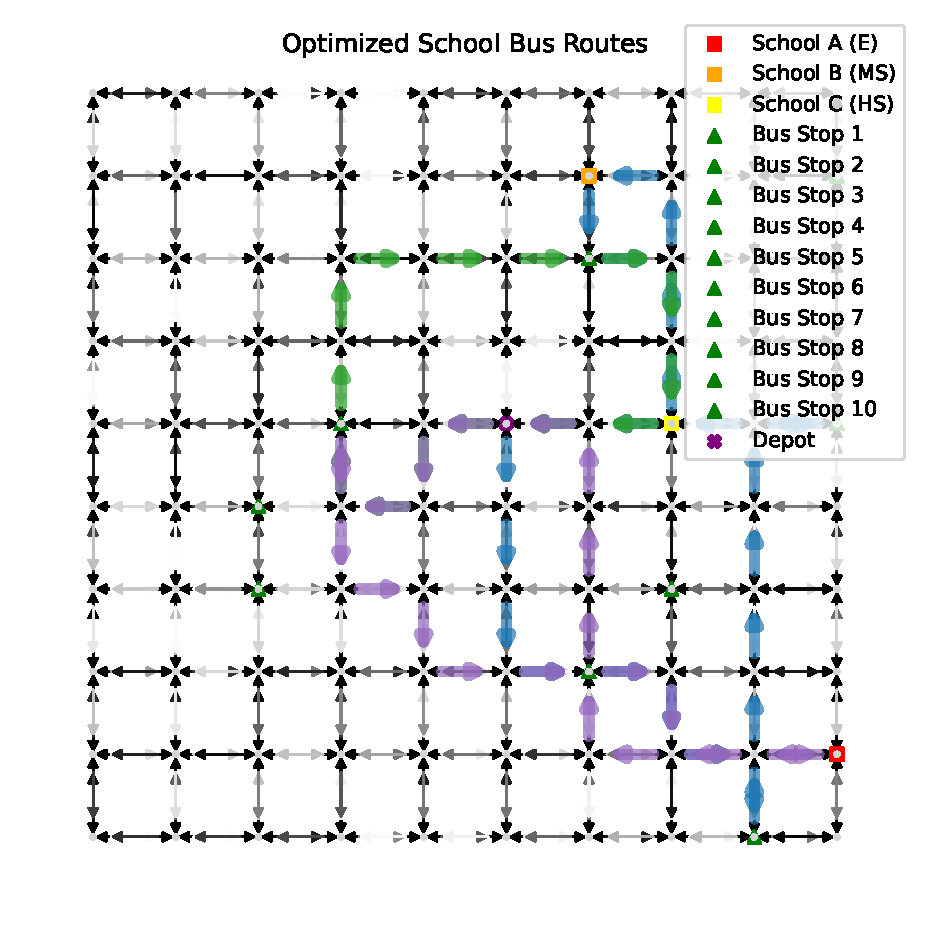
\includegraphics[width=0.5\linewidth, alt={Grid-based toy network with random edge weights showing optimized school bus routes. Colored route segments connect selected stops to schools and a depot, demonstrating that the routing formulation can generate feasible bus paths on a small artificial network.}]{figures/initial_test.pdf}
    \caption{Initial test of bus routing in a 10 by 10 toy network, using 3 schools of different types, 1 central depot, and 10 total bus stops. Each directed edge has a random weight assigned.}
    \label{fig:placeholder}
\end{figure}

The co-design composition enables a clear separation between physical and institutional subsystems while maintaining their properties. For example, a fleet component maps a set of buses $\mathcal{B}$ with capacities $C_b$, ranges $R_b$, and accessibility attributes $W_b$ to feasible routing capabilities. Meanwhile, a staffing component models the availability of monitors and drivers, and a policy component encodes equity objectives such as sufficient coverage for particular demographic groups. These components are combined into a global design problem, whose solution set can be projected onto different objective spaces like cost or coverage, to generate explicit Pareto frontiers. These allow planners and stakeholders to weigh distinct tradeoffs between different possible solutions and configurations.

\section{Data Sources and Preprocessing}

I utilize network, operational, demand, and demographic information and format it into a common mathematical representation. The physical road network is obtained from \gls{osm} and converted into a directed graph $\mathcal{G}=\left\langle\mathcal{V},\mathcal{E},\omega\right\rangle$, where nodes $\mathcal{V}$ represent intersections, depots, stops, and schools. Directed edges $\mathcal{E}$ capture feasible roadway movements with associated attributes $\omega_e$ such as length, speed, and travel time. From this base graph, I identify the subset of nodes corresponding to bus pick-up locations $\mathcal{P}$, destination locations $\mathcal{S}$, and bus depot locations $\mathcal{D}$ using geocoded address records and provided facility data.

\gls{gtfs} data can provide scheduled trip patterns, stop locations, and route identifiers for the existing network, which are linked to \gls{osm}-derived nodes. If available, \gls{avl} traces that are representative of a given area are cleaned and matched to the road network to estimate real-world travel times. These estimates are then aggregated for every edge and time-of-day and used to define the travel-time component of $\omega_e$.

Demand is represented as a set of individuals $\mathcal{M}$, each associated with a pickup stop $p_m\in \mathcal{P}$, an assigned destination school $s_m\in \mathcal{S}$. For the case study, I additionally employ a school type $\tau_m\in \mathcal{T}$ that encodes the grade levels served by a school (elementary, middle, or high school). Additionally, one can exclude students that reside within a fixed walking threshold $\gamma$ of their destination school by computing network shortest-path distances from each school to nearby residential locations and filtering those below $\gamma$. 

Demographic attributes from the \gls{acs}, such as income distribution, race and ethnicity composition, English proficiency, and car access, are joined to student and stop nodes via census block groups, which can later be used as equity indicators when evaluating Pareto-optimal designs. Due to the need for data precision, this work used \gls{acs} 2020--2024 5-year estimates to provide the most accurate and granular data, particularly due to the usage of small geographies like block groups.

I also incorporate student-level indicator functions to flag the need for additional on-board support and wheelchair accessibility. A binary flag $f_m$ identifies students in set $\mathcal{F}\subseteq\mathcal{M}$ who require a monitor, and a subset $\mathcal{W}\subseteq\mathcal{F}$ identifies those who require a wheelchair-accessible bus. These attributes are derived from the district's special education transportation records and are used to enforce monitor and vehicle constraints at the routing stage. 

\section{Co-Design and \Glsentryfull{milp} Formulation}

\begin{figure}[!htbp]
    \centering
    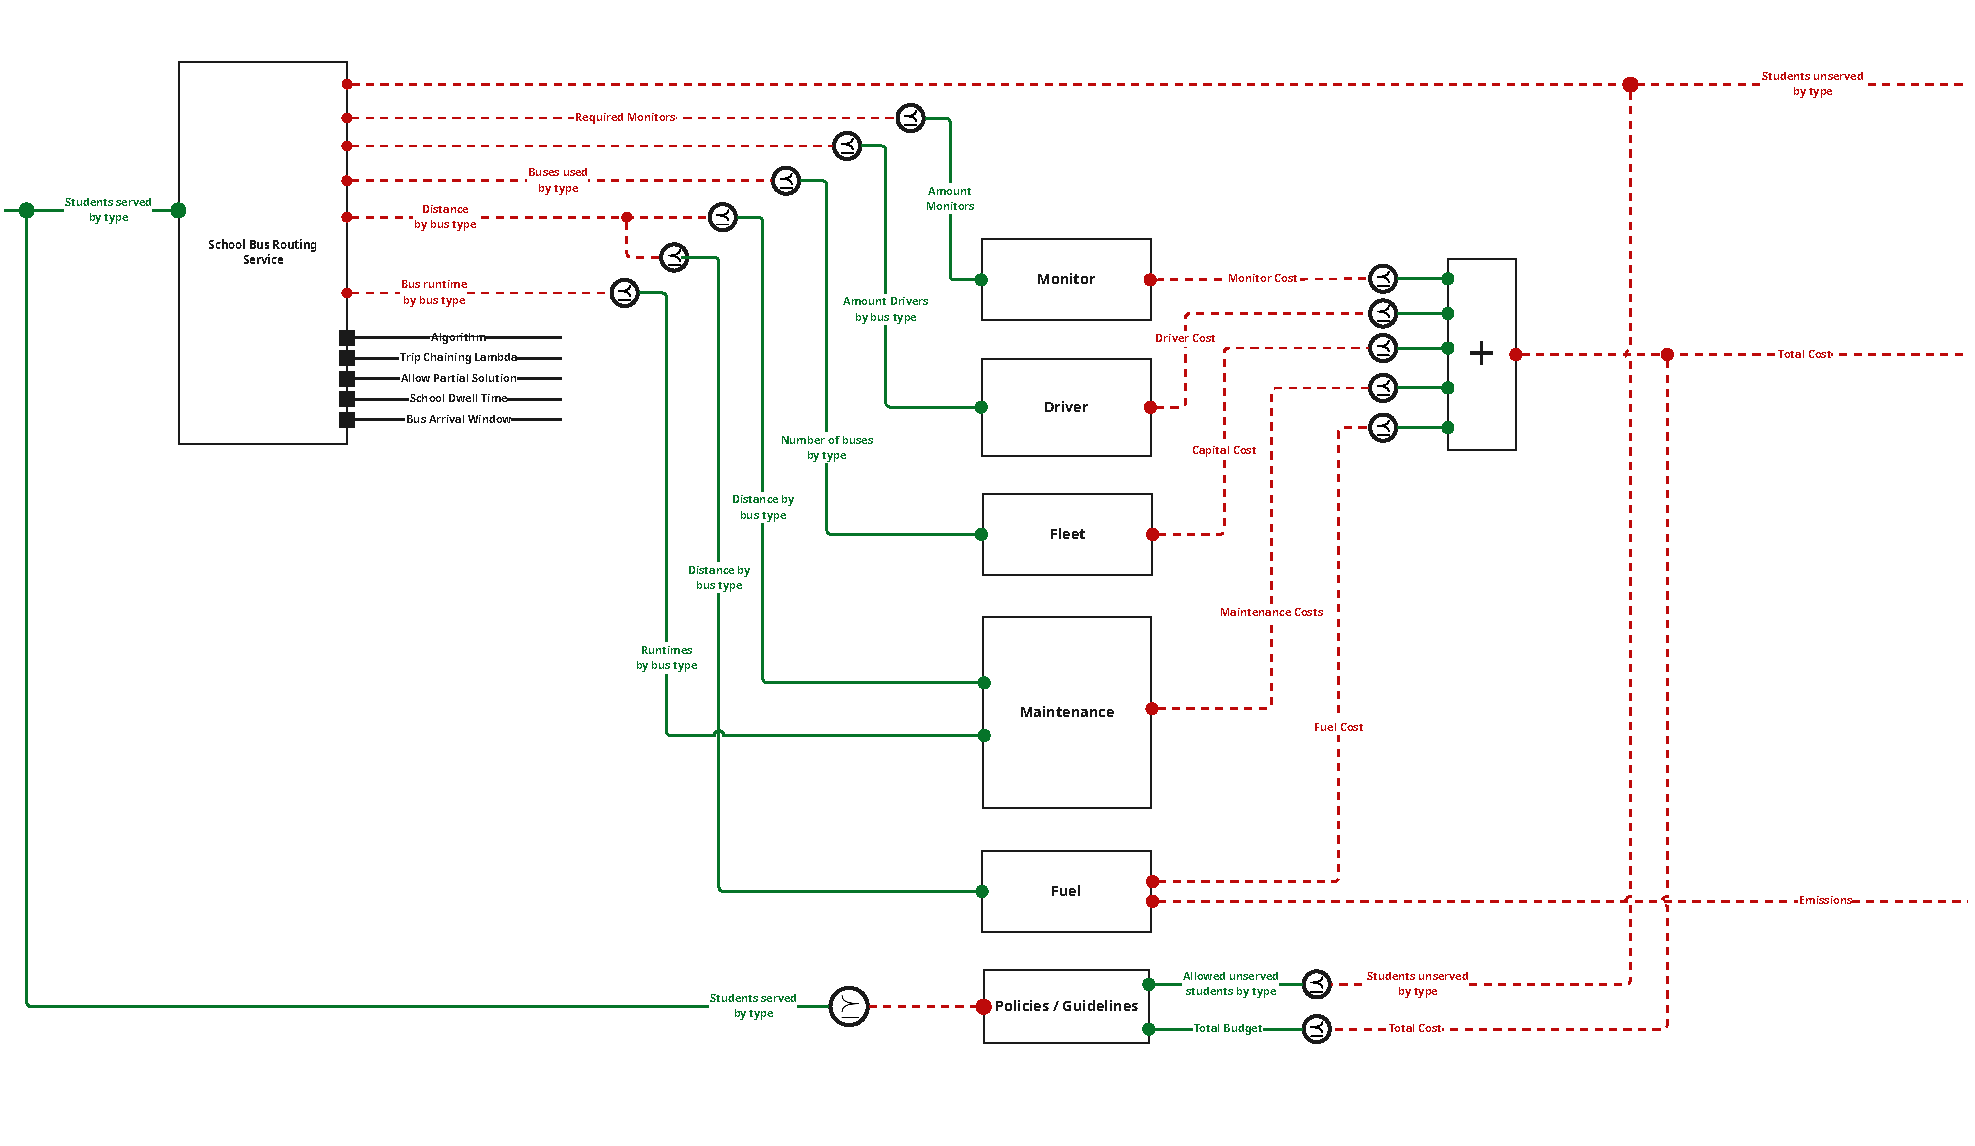
\includegraphics[width=0.99\linewidth, alt={Co-design system diagram showing how routing service inputs, bus capacity, driver, fuel, maintenance, monitor, and routing algorithm parameters connect to outputs such as total cost, unserved students, stops used, emissions, and accessibility-related service metrics.}]{figures/codesign_diagram_simple.pdf}
    \caption{Simplified co-design diagram, illustrating how different components and their respective functionalities (in green) and requirements (in red) interact.}
    \label{fig:codesign}
\end{figure}

\autoref{fig:codesign} summarizes the resulting co-design composition, with each box representing an \gls{mdpi} (monitor, bus capacity, driver, fuel, maintenance, and routing service) connected via respective functionalities and resources. At the core of this framework is a sequential pipeline of \glspl{milp} that encodes the routing and assignment decisions. This can be tailored to a specific use case, and below is a formulation for the specific Framingham case study. The full, original formulation below is presented as background motivation; due to computational intensity, the implementation that follows uses a modified \gls{bird} backend presented in \cite{delarueOptimizing}.

\subsection{Initial Formulation}
\label{sec:original_milp}

In the original formulation, the \gls{milp} chooses which buses to use, what arcs they traverse, and which students they carry, while simultaneously respecting capacity, maximum ride time, and school arrival windows. It does this while also attempting to minimize a weighted sum of distances and bus/monitor usage. 

The routing network is defined by routing nodes $\mathcal{N}\coloneq\mathcal{P}\cup\mathcal{S}\cup\mathcal{D}^{+}\cup\mathcal{D}^{-}\cup\mathcal{S}^{+}$ and directed arcs $\mathcal{A}\subseteq \mathcal{N}\times\mathcal{N}$, where each arc $\left(i,j\right)\in\mathcal{A}$ represents travel along a (precomputed) shortest path in $\mathcal{G}$ with distance $d_{ij}$ and travel time $t_{ij}$. To model multi-round ``trip chaining'' for each bus, I introduce a set of rounds $\mathcal{Q}=\left\{1,\ldots,Q^{\max}\right\}$, where each round represents a sub-tour that begins at a node and ends either at a school or at the depot. This can be used to reflect a ``multi-tiered'' trip system, while ensuring that the initial round must begin at the depot and the final round must end at the depot.

Decision variables in the \gls{milp} include $z_b$ for whether bus $b$ is used, $z_{b,q}$ for whether bus $b$ operates in round $q$, and $x_{b,q,ij}$ for whether bus $b$ traverses arc $\left(i,j\right)$ in round $q$. The variables $v_{b,q,i}$ are introduced to indicate whether node $i$ is visited by bus $b$ in round $q$, and $e_{b,q,s}$ record whether round $q$ for bus $b$ ends at school $s$, enabling trip chaining via school start-copy nodes $s^{+}$ for subsequent rounds. Student bus assignments are represented by $a_{m,b,q}$, which equals 1 if student $m$ is on bus $b$ in round $q$. These variables enforce that each student is assigned to at most one bus and one round and that all students are served when the coverage ratio $\phi$ is set to 1.

Time and capacity constraints are captured using continuous variables $T_{b,q,i}$ for the arrival time of bus $b$ at node $i$ in round $q$, and integer variables $L_{b,q,i}$ for the on-board passenger load immediately after visiting node $i$. Alighting and boarding service times are set through user defined constant parameters $\alpha=0.3$ minutes per boarding and $\beta=0.5$ minutes per alighting, which both contribute additively to the time-linking constraints on arcs and to the chaining of rounds at schools. To handle differences in school types and bus capacity for different ages, the \gls{milp} formulation also includes binary variables $y_{b,q,\tau}$ specifying the active school type $\tau\in\mathcal{T}$ for each bus and round, along with a multiplier $\kappa_\tau$ that scales the functional capacity of bus $b$ according to the served school type (e.g. elementary school students can fit 3 to a seat compared to 2 for middle and high schoolers).

The objective function minimizes a weighted sum of total distance traveled across buses, an optional per-round tiebreaker, and an indicator for using buses with monitors (which increases labor cost). Specifically, the primary term sums distances $d_{ij}$ over all active arcs $x_{b,q,ij}$, while a small penalty $\lambda^{\mathrm{round}}$ is applied to $z_{b,q}$ to discourage unnecessary tour fragments (without overriding distance minimization when $\lambda^{\mathrm{round}}$ is small). An additional term $r_b^{\mathrm{mon}}$ indicates whether bus $b$ carries a monitor (along with a penalty term $\lambda^{\mathrm{mon}}$), which allows the optimization to incorporate monitor staffing costs or prioritize configurations that reduce monitor deployment (while still meeting all special transportation constraints) by summing across all buses.

\[
\min{\sum_{b\in\mathcal{B}} \sum_{q\in\mathcal{Q}} \sum_{\left(i,j\right)\in\mathcal{A}} d_{ij} x_{b,q,ij} + \lambda^{\mathrm{round}} \sum_{b\in\mathcal{B}} \sum_{q\in\mathcal{Q}} z_{b,q} +\lambda^{\mathrm{mon}} \sum_{b\in\mathcal{B}} r_{b}^{\mathrm{mon}}}
\]

These constraints together enforce student assignment coverage, tour feasibility, time consistency, max time limits, capacity adherence, and monitor and wheelchair-accessibility requirements. Assignment constraints ensure each student is assigned at most once and that the aggregate number of assigned students meets the desired coverage $\phi\left\vert\mathcal{M}\right\vert$.

\[
\sum_{b\in\mathcal{B}} \sum_{q\in\mathcal{Q}} a_{m,b,q} \leq 1 \qquad \forall m\in\mathcal{M}
\]
\[
\sum_{m\in\mathcal{M}}\sum_{b\in\mathcal{B}} \sum_{q\in\mathcal{Q}} a_{m,b,q} \geq \phi\left\vert\mathcal{M}\right\vert
\]

Flow-conservation and depot/school connection constraints also ensure that each round is a valid tour. This is enforced through $z_{b,q}$, $v_{b,q,i}$, and $x_{b,q,ij}$, and the full indexing details are omitted for readability.

Time-linking constraints guarantee that arrival times along arcs respect travel plus dwell times and that buses depart schools for the next round only after boarding/alighting. Latest-arrival constraints require that the arrival time at each school $s$, plus the relevant alighting dwell, does not exceed the latest allowable arrival $\ell_s=h_s-\delta_s$, where $h_s$ is the bell time (represented as minutes from midnight) and $\delta_s$ is a required slack.

\[
T_{b,q,j} \geq T_{b,q,i} + t_{ij}
+ \mathrm{service}_i
- M^{\mathrm{time}}\left(1-x_{b,q,ij}\right) \qquad \forall b\in\mathcal{B},\forall q\in\mathcal{Q},\forall \left(i,j\right)\in\mathcal{A}
\]
\[
\mathrm{service}_i=\alpha \sum_{m\in\mathcal{M}:p_m=i} a_{m,b,q}
+ \beta \sum_{m\in\mathcal{M}:s_m=i} a_{m,b,q} \qquad \forall b\in\mathcal{B},\forall q\in\mathcal{Q}
\]
\[
T_{b,q,s} + \beta\sum_{m\in\mathcal{M}:s_m=s} a_{m,b,q} \leq \ell_s + M^{\mathrm{time}}\left(1-v_{b,q,s}\right) \qquad \forall b\in\mathcal{B},\forall q\in\mathcal{Q},\forall s\in\mathcal{S}
\]

To control individual student experiences, precedence constraints enforce that a student’s school is visited after their pickup stop by at least a small separation $\epsilon$, and ride-time constraints require that the difference $T_{b,q,s_m}-T_{b,q,p_m}$ does not exceed an arbitrary maximum in-vehicle time $H^{\mathrm{ride}}$ when $a_{m,b,q}=1$.

\[
T_{b,q,s_m} - T_{b,q,p_m}
\leq H^{\mathrm{ride}} + M^{\mathrm{time}}\left(1-a_{m,b,q}\right) \qquad \forall b\in\mathcal{B},\forall m\in\mathcal{M},\forall q\in\mathcal{Q}
\]

Capacity dynamics are handled by linking the load variables $L_{b,q,i}$ across arcs by using the number of students boarding or alighting at each node and bounding the load by the actual capacity $C_b\sum_{\tau}\kappa_\tau y_{b,q,\tau}$. Additional constraints set loads to zero at depots and school start-copy nodes to reset tours, as well as ensure that ending a final round at a school implies an empty bus at that school. 

\[
0 \leq L_{b,q,i} \leq C_b \sum_{\tau\in\mathcal{T}} \kappa_{\tau} y_{b,q,\tau} \qquad \forall b\in\mathcal{B},\forall q\in\mathcal{Q},\forall i\in\mathcal{N}
\]

Monitor-related constraints couple the presence of flagged students $m\in\mathcal{F}$ with the binary variable $r_b^{\mathrm{mon}}$, making sure that any bus carrying a flagged student in any round also carries a monitor, and also that wheelchair-using students $m\in\mathcal{W}$ can only be assigned to buses with $W_b=1$.

\[
a_{m,b,q} \leq r_b^{\mathrm{mon}} \qquad \forall m\in\mathcal{F},\forall b\in\mathcal{B},\forall q\in\mathcal{Q}
\]
\[
a_{m,b,q} \leq W_b \qquad \forall m\in\mathcal{W},\forall b\in\mathcal{B},\forall q\in\mathcal{Q}
\]

\begin{figure}[!htbp]
    \centering
    \begin{subfigure}{0.495\textwidth}
        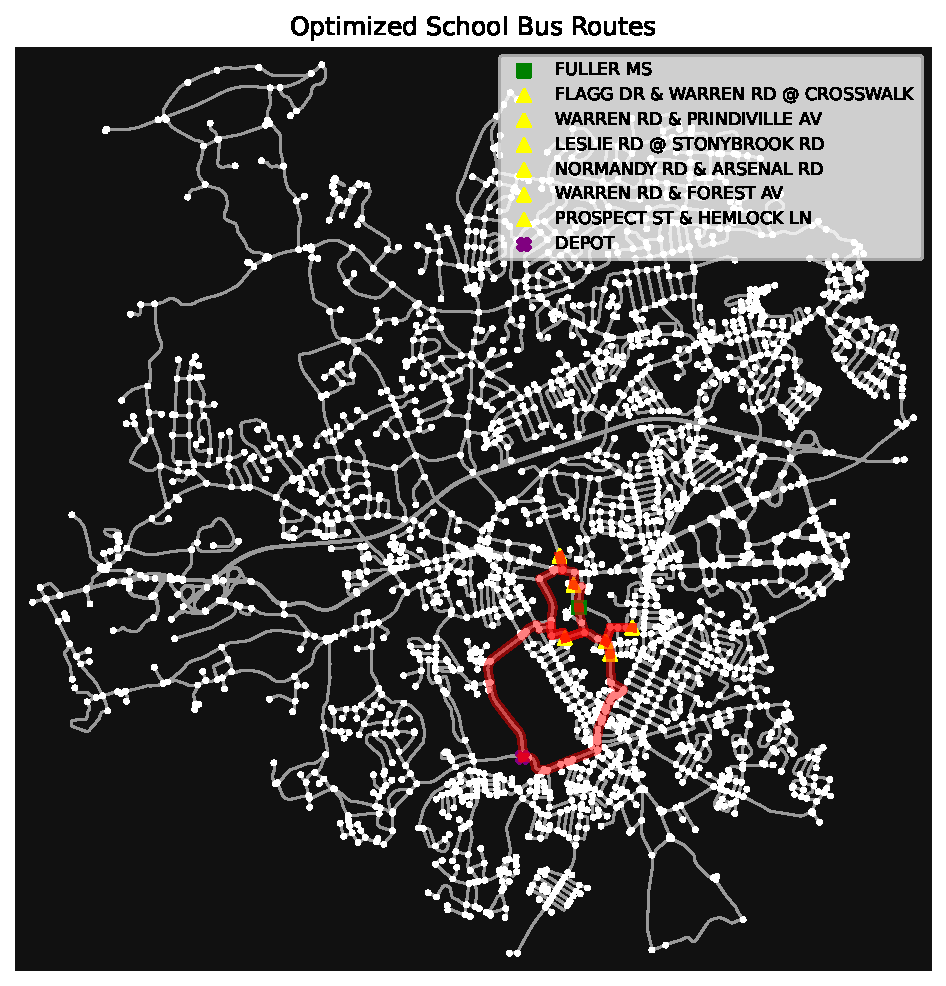
\includegraphics[width=0.99\textwidth, alt={Map of initial optimized bus routes for students within one kilometer of a school, without trip chaining. Red route segments show the selected bus path over the Framingham road network.}]{figures/no_chaining_routes.pdf}
        \subcaption{Route serving all students within 1 kilometer of a school without chaining ($Q^{\max}=1$)}
    \end{subfigure}
    \begin{subfigure}{0.495\textwidth}
        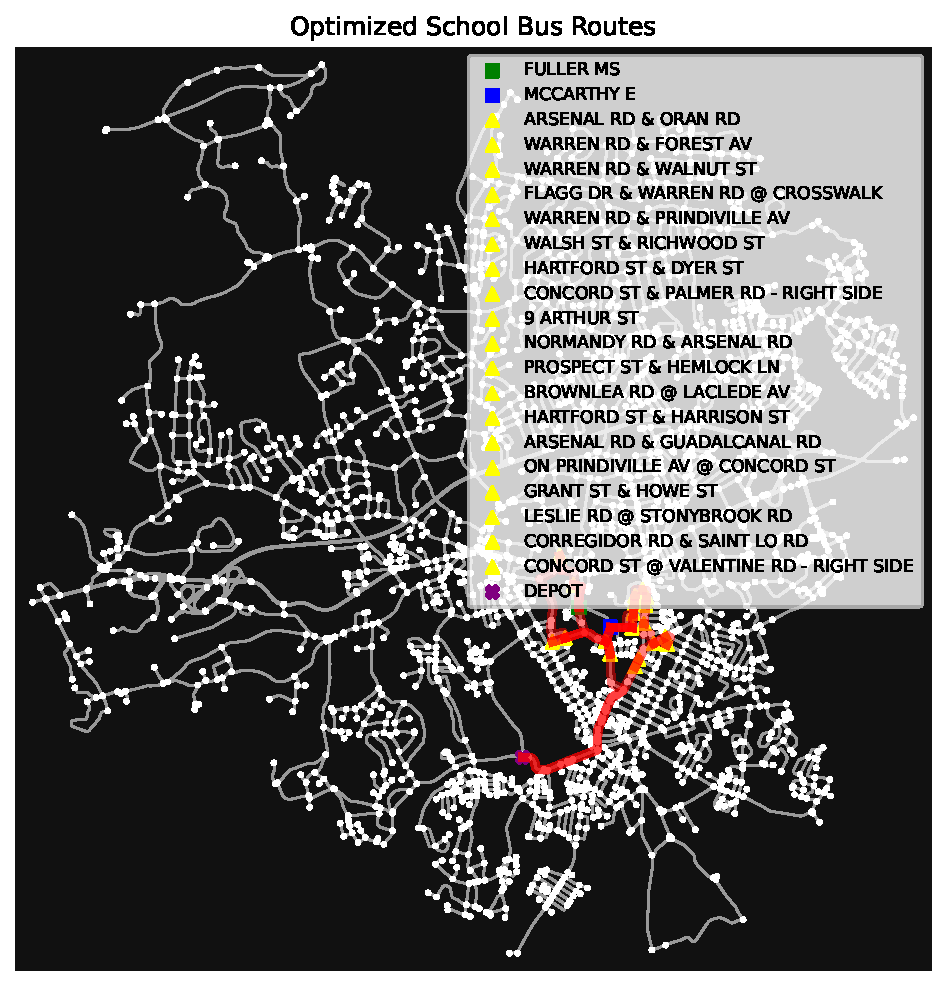
\includegraphics[width=0.99\textwidth, alt={Map of initial optimized bus routes for students within one kilometer of two schools, with trip chaining. Red route segments show the selected bus path over the Framingham road network.}]{figures/chaining_routes.pdf}
        \subcaption{Route serving all students within 1 kilometer of 2 schools using a single bus ($Q^{\max}=2$)}
    \end{subfigure}
    \caption{Initial test routes using the original formulation}
    \label{fig:prelim_results}
\end{figure}

While this initial formulation was able to handle small networks well as shown in \autoref{fig:prelim_results}, this became computationally prohibitively expensive as the problem size increased: approximately 30 stops with 1 school failed to solve in a reasonable amount of time. This is due to the large quantity of simultaneous constraints, particularly as individual sets expanded to the size of a full city, which led us to consider a decomposed formulation that completes the routing problem in stages like \gls{bird}. 

\subsection{\Glsentryfull{bird} Backend}

Rather than implementing a new formulation from scratch, an adapter that ingests the sets described in \autoref{sec:original_milp} is passed to a modified \gls{bird} backend that provides two main routing algorithms: a scenario-based optimization method and a constructive \gls{lbh}, denoted as \verb!scenario! and \verb!lbh!. Both methods operate on the same underlying  representation, which stores schools, stops, student assignments, fleet attributes, travel times, bell times, and special transportation requirements. However, they differ in how they search the feasible design space.

The \verb!scenario! method follows a generate-and-optimize structure. First, it constructs a large pool of feasible candidate routes using greedy nearest-insertion procedures under multiple different parameter settings. These configurations are the ``scenarios'' in the implementation: alternative route-generation settings used to vary the candidate pool. Each candidate route serves a single school $s$ and already satisfies local feasibility constraints such as vehicle capacity, school arrival timing, student ride-time limits, and special transportation restrictions. The second stage then solves a \gls{milp} that selects from this candidate set. In the homogeneous case, this resembles a set-covering formulation in which binary route-selection variables cover required stops while minimizing a weighted route cost. In the fleet-aware case, the model additionally assigns selected routes to specific buses, tracks bus usage, and permits chaining multiple school routes onto a single vehicle when the resulting arrival and departure times remain feasible.

The fleet-aware \verb!scenario! formulation is therefore a decomposed alternative to the full arc-based \gls{milp} described in \autoref{sec:original_milp}. Rather than deciding every street-level arc traversal directly, it optimizes over complete feasible route candidates. The model includes variables indicating whether a bus is used, whether a route is assigned to a bus, whether a route begins or ends a bus itinerary, and whether two routes can be linked consecutively by the same bus. Sparse linking variables encode only temporally feasible route-to-route transitions, reducing the number of impossible chaining decisions considered by the solver. The implementation also solves the problem in \textit{service groups}, routing wheelchair-accessible students first, then students requiring transportation with staff monitors, and finally students without additional transportation needs. This structure reflects operational priority constraints, while still allowing later stages to use remaining fleet capacity.

The \verb!lbh! method provides a faster solver-free baseline. Instead of generating many routes and solving a mixed-integer selection problem, it constructs bus itineraries directly through repeated cheapest insertion. Here, buses are considered in capacity-priority order, and the algorithm inserts uncovered stops into the current itinerary whenever doing so preserves capacity, grade compatibility, maximum ride-time, and school timing feasibility. For fixed bell-time schools, insertions are evaluated against a fixed arrival constraint; for schools with allowable time windows, the insertion logic also accounts for the flexibility of the arrival window. As in the scenario-based method, the fleet-aware heuristic proceeds through wheelchair, monitor-required, and conventional service groups.

These two modes expose a useful quality-runtime tradeoff. The \verb!scenario! method is slower and requires a \gls{milp} solver, but it can make globally coordinated decisions over a diverse pool of candidate routes and explicitly optimize route chaining across a heterogeneous fleet. The \verb!lbh! method is substantially faster and does not require a solver, but it makes myopic decisions: once a stop insertion or bus assignment is made, the algorithm does not globally reconsider that choice. In the framework, \verb!scenario! is therefore used when higher-quality optimized designs are desired, while \verb!lbh! provides a computationally lightweight benchmark and fallback routing procedure. These modes can be queried to compute an implementation catalog of solutions, which can then be ingested by \gls{mcdp}. Pareto fronts created using this method and testing data can be seen in \autoref{fig:bird_simple}.

\begin{figure}[!htbp]
    \centering
    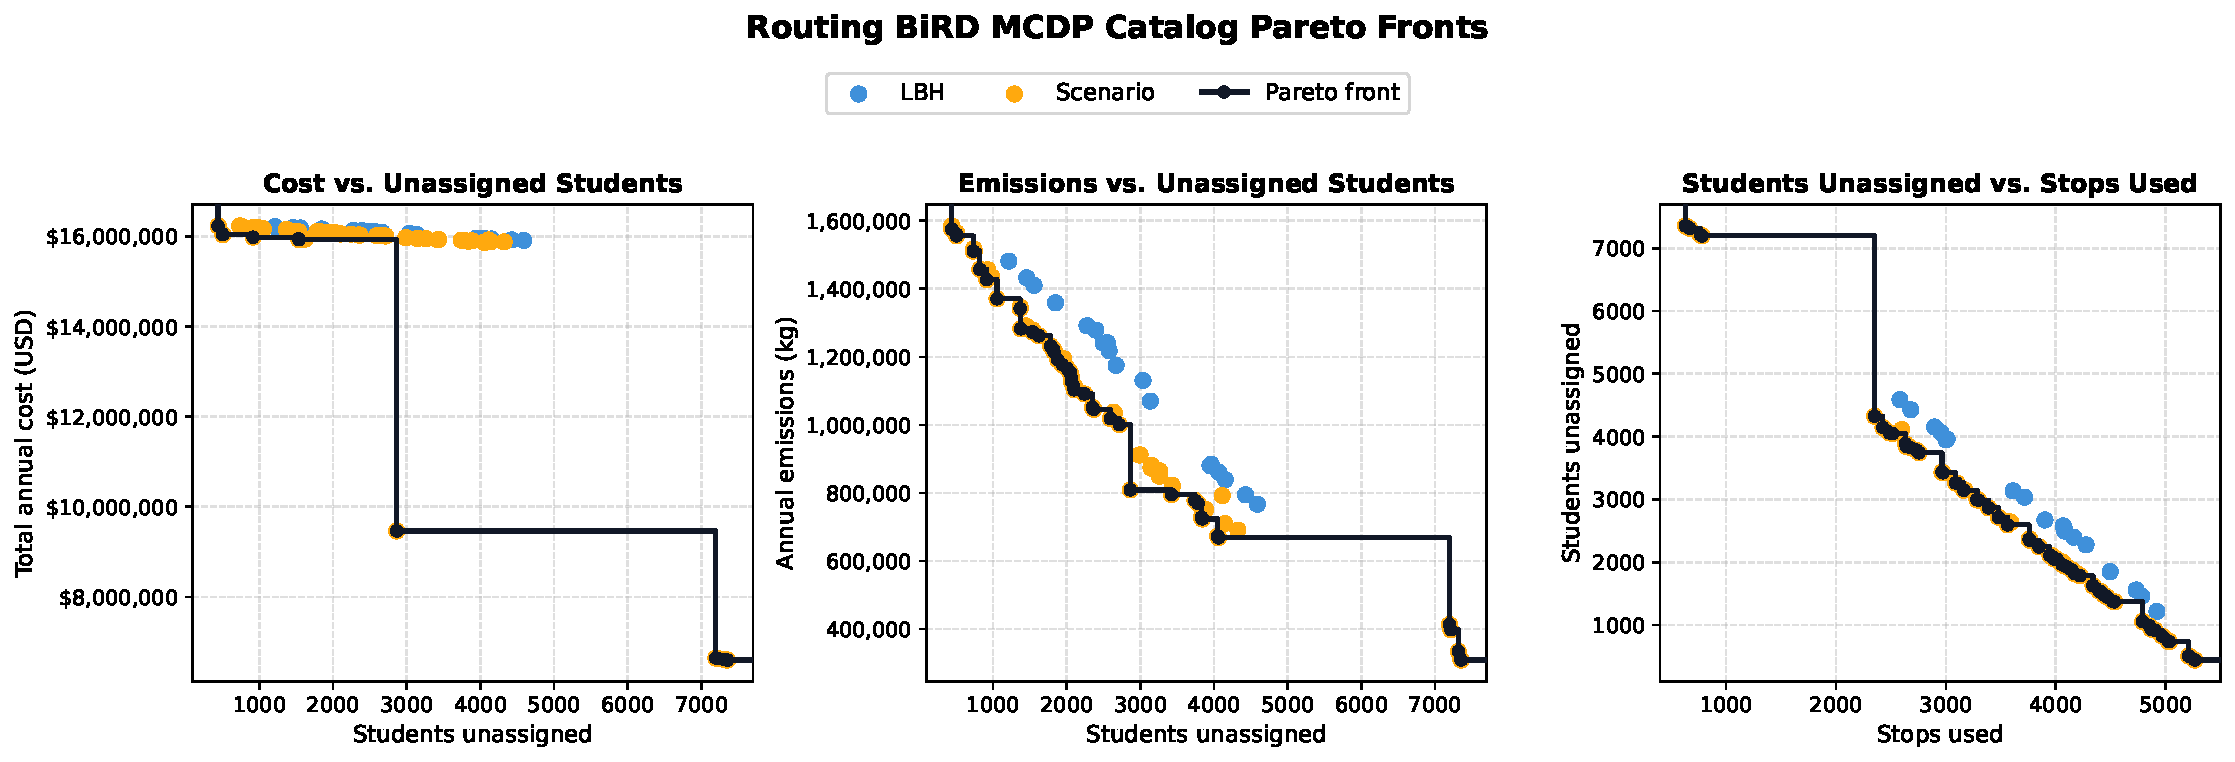
\includegraphics[width=0.99\linewidth, alt={Three side-by-side Pareto-front scatter plots comparing \glsentrylong{lbh} and Scenario \glsentrylong{bird} outputs on catalog data. The plots show tradeoffs between unassigned students and cost, unassigned students and annual emissions, and unassigned students and stops used. Blue points represent \glsentrylong{lbh} solutions, red points represent scenario solutions, and the black line marks the Pareto frontier.}]{figures/routing_bird_mcdp_pareto_all.pdf}
    \caption{Pareto fronts using sampled \gls{bird} routes with different possible catalog configurations.}
    \label{fig:bird_simple}
\end{figure}

\section{Case Study Implementation for Framingham}

I implement the framework described for the Framingham, Massachusetts school bus system to illustrate its practical use in evaluating and redesigning a real-world network. The case study for \gls{fps} focuses on morning school arrivals for a single day representative of regular operations, using district-provided data on student assignments, current route structures, fleet composition, and special transportation requirements. \Gls{fps} provided the core datasets required to conduct a preliminary routing analysis: school locations, schools served, school start times, student home locations, assigned schools, grade levels, current bus assignment, and fleet characteristics, including bus size, capacity, and type. \gls{fps} also confirmed that all buses operate from a single central depot and that current school transportation is planned independently of the local public transportation provider, \gls{mwrta}. Accordingly, \gls{mwrta} service is excluded from this analysis.

To begin, I map the provided data into the sets and parameters for \gls{bra}, including the actual fleet $\mathcal{B}$, bus depot set $\mathcal{D}$, school set $\mathcal{S}$, and student set $\mathcal{M}$ with flags $\mathcal{F}$ and $\mathcal{W}$. This allows for comparisons between existing routes and generated ones, producing a feasible design point that reflects the existing system.

I use \gls{osm} to model the road network and connect it with existing depot, stop, and school locations. The \gls{osm}-derived Framingham road network used to construct travel arcs is shown in \autoref{fig:framingham}. Based on walking distances computed using \textcite{fink2022R5py}, students are assigned to their closest stops (or for students currently served, the current assignment is imposed). Given the available bus fleet, school bell/start times, a manually set time window before these bell times, and a maximum in-vehicle ride-time (here set to 60 minutes), I then generate a family of alternative feasible designs based on the described \gls{bra}, adapting the decomposition approach of \textcite{bertsimasOptimizingSchoolsStart2019}. 


\begin{figure}[!htbp]
    \centering
    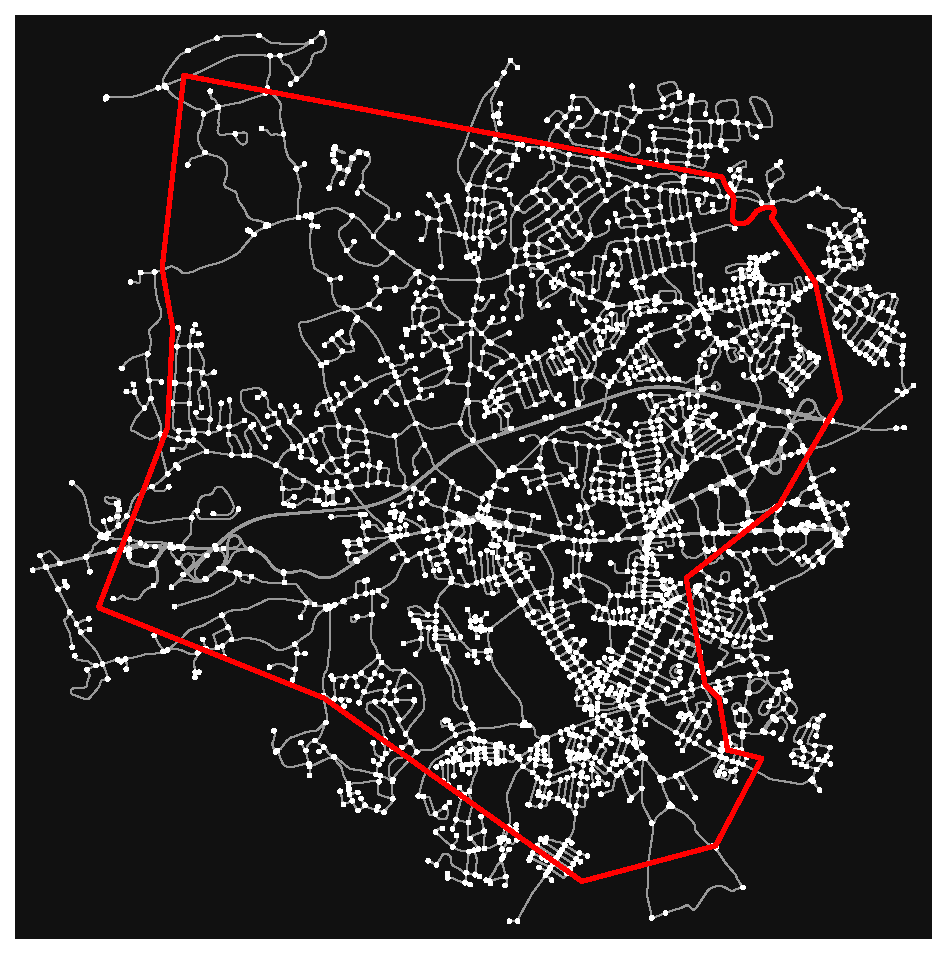
\includegraphics[width=0.5\linewidth, alt={Map of the Framingham road network used to construct travel arcs. White road segments appear on a dark background, with a red boundary outlining the study area.}]{figures/framingham.pdf}
    \caption{Current Framingham road network used to create travel arcs}
    \label{fig:framingham}
\end{figure}

The available data is sufficient to identify and assess the current routing and test alternative configurations, but it is not yet sufficient for final implementation. The key limitation is that the dataset for currently served students includes assigned stops and disability status, but these records cannot be directly linked to each student's home address. This prevents full validation of current stop assignments and limits the precision of student-level service comparisons.

Because \gls{fps} was not yet able to provide real-world \gls{avl} data, \gls{bra} assumes a fixed driving speed of 30 miles per hour, incorporating boarding and alighting times of the various student groups (including students with disabilities, students requiring wheelchair-accessible routes, and students without additional transportation needs), and allows for multiple rounds by the same bus, dropping off students at one school before picking up additional students and bringing them to another school. To do so, this approach first allocates routes to students requiring accessible routes and students with disabilities, then caters to the remaining students.

The categorical co-design framing shaped the Framingham experiments by treating routing as a compositional feasibility problem: district resources, service requirements, accessibility constraints, and environmental costs are modeled as interconnected design variables rather than as a single monolithic objective. The Pareto fronts therefore represent the feasible tradeoff surface exposed by this design space, showing how changes in one component, such as fleet use, stop coverage, or student service, propagate through the broader transportation system. The \gls{mcdp} constructed and used in this thesis is described in formal detail in \hyperref[ap:mcdpl]{Appendix~\ref*{ap:mcdpl}}.

The experiments in \autoref{ch:results} evaluate this pipeline in three increasingly expansive service scenarios: the current set of assigned \gls{fps} riders, students living at least 1.5 miles from school, and the full student population. For each scenario, \gls{bra} produces route candidates and evaluates the resulting designs using fleet use, student coverage, estimated ride time, route density, cost, emissions, and Pareto-front position. Because \gls{avl} traces and complete student-stop-home linkages were not available, these outputs should be interpreted as comparative planning estimates rather than deployment-ready schedules.

\begin{nomenclature*}[2em][Nomenclature for Chapter \ref*{ch:methods}][section]
    \EntryHeading{Sets and indices}
    \entry{$\mathcal{G}$}{\gls{osm}-derived directed road graph with edge attributes, $\mathcal{G}=\left\langle\mathcal{V},\mathcal{E},\omega\right\rangle$}
    \entry{$\mathcal{V}$}{Road-network nodes, including intersections, stops, depots, and schools}
    \entry{$\mathcal{E}$}{Directed road-network edges}
    \entry{$\omega_e$}{Attribute vector for road edge $e$, such as length, speed, and travel time}
    \entry{$\mathcal{P}$}{Pickup-stop nodes}
    \entry{$\mathcal{S}$}{School or destination nodes}
    \entry{$\mathcal{S}^{+}$}{School or destination start-copy nodes used for trip chaining}
    \entry{$\mathcal{D}$}{Depot nodes used in routing}
    \entry{$\mathcal{D}^{+}$}{Depot start-copy nodes}
    \entry{$\mathcal{D}^{-}$}{Depot end-copy nodes}
    \entry{$\mathcal{N}$}{Routing nodes, $\mathcal{P}\cup\mathcal{S}\cup\mathcal{D}^{+}\cup\mathcal{D}^{-}\cup\mathcal{S}^{+}$}
    \entry{$\mathcal{A}$}{Directed routing arcs between routing nodes}
    \entry{$\mathcal{M}$}{Students or riders represented in the demand set}
    \entry{$\mathcal{F}$}{Students requiring a staff monitor}
    \entry{$\mathcal{W}$}{Students requiring wheelchair-accessible service}
    \entry{$\mathcal{B}$}{Bus fleet}
    \entry{$\mathcal{Q}$}{Ordered trip-chaining rounds, $\mathcal{Q}=\left\{1,\ldots,Q^{\max}\right\}$}
    \entry{$\mathcal{T}$}{School or grade-level types, such as elementary, middle, and high school}
    \EntryHeading{Parameters}
    \entry{$d_{ij}$}{Shortest-path distance for routing arc $\left(i,j\right)$}
    \entry{$t_{ij}$}{Travel time for routing arc $\left(i,j\right)$}
    \entry{$p_m$}{Pickup stop assigned to student $m$}
    \entry{$s_m$}{School assigned to student $m$}
    \entry{$\tau_m$}{School or grade-level type for student $m$}
    \entry{$\gamma$}{Walking-distance eligibility threshold}
    \entry{$\alpha$}{Boarding service time per student}
    \entry{$\beta$}{Alighting service time per student}
    \entry{$C_b$}{Nominal capacity of bus $b$}
    \entry{$\kappa_\tau$}{Capacity multiplier for school type $\tau$}
    \entry{$W_b$}{Indicator that bus $b$ is wheelchair-accessible}
    \entry{$h_s$}{Bell time or required arrival time for school $s$}
    \entry{$\delta_s$}{Required arrival slack before bell time at school $s$}
    \entry{$\ell_s$}{Latest allowable arrival time at school $s$, $\ell_s=h_s-\delta_s$}
    \entry{$H^{\mathrm{ride}}$}{Maximum in-vehicle ride time}
    \entry{$\epsilon$}{Minimum separation used in pickup-before-dropoff precedence constraints}
    \entry{$\phi$}{Required coverage ratio}
    \entry{$\lambda^{\mathrm{round}}$}{Penalty for unnecessary route fragments or rounds}
    \entry{$\lambda^{\mathrm{mon}}$}{Penalty or cost weight for monitor use}
    \EntryHeading{Decision variables}
    \entry{$z_b$}{1 if bus $b$ is used}
    \entry{$z_{b,q}$}{1 if bus $b$ operates in round $q$}
    \entry{$x_{b,q,ij}$}{1 if bus $b$ traverses routing arc $\left(i,j\right)$ in round $q$}
    \entry{$v_{b,q,i}$}{1 if bus $b$ visits node $i$ in round $q$}
    \entry{$e_{b,q,s}$}{1 if round $q$ for bus $b$ ends at school $s$}
    \entry{$a_{m,b,q}$}{1 if student $m$ is assigned to bus $b$ in round $q$}
    \entry{$T_{b,q,i}$}{Arrival time of bus $b$ at node $i$ in round $q$}
    \entry{$L_{b,q,i}$}{Passenger load on bus $b$ after visiting node $i$ in round $q$}
    \entry{$y_{b,q,\tau}$}{1 if bus $b$, round $q$, is assigned to school type $\tau$}
    \entry{$r_b^{\mathrm{mon}}$}{1 if bus $b$ carries a staff monitor}
\end{nomenclature*}
